
%(BEGIN_QUESTION)
% Copyright 2015, Tony R. Kuphaldt, released under the Creative Commons Attribution License (v 1.0)
% This means you may do almost anything with this work of mine, so long as you give me proper credit

A safety device commonly installed on process vessels containing pressurized gases is a {\it Pressure Safety Valve}, or PSV.  In this example, a PSV protects a reactor vessel against rupture from excessive internal gas pressure, with the PSV set to open (``lift'') and vent the tank if the internal pressure exceeds 77 PSI:

$$\includegraphics[width=15.5cm]{i00502x01.eps}$$

Calculate the total force exerted on a 14 inch blind flange located on the side of the reactor at the PSV lift pressure, both in pounds and in tons.  Use 13$1 \over 4$ inches as the effective diameter of the blind flange.

\vskip 10pt

$F_{total}$ = \underbar{\hskip 50pt} lb

\vskip 10pt

$F_{total}$ = \underbar{\hskip 50pt} tons

\vskip 20pt \vbox{\hrule \hbox{\strut \vrule{} {\bf Suggestions for Socratic discussion} \vrule} \hrule}

\begin{itemize}
\item{} If this reactor vessel held a liquid instead of a gas, would it affect the calculations of force applied to the flange?  Why or why not?
\item{} If this reactor vessel held a liquid instead of a gas, would it affect the proper selection of the overpressure valve?  Why or why not?
\item{} If this reactor vessel's temperature were to substantially increase, would it affect the proper overpressure valve setting?  Why or why not?
\item{} If this reactor's fluid were extremely flammable and/or toxic, what would be the safest way to plumb an overpressure valve, since direct release to the atmosphere would be itself unsafe?
\item{} A dangerous practice unfortunately seen in some industries is called {\it hot-bolting} of flanges, where only half of the flange bolts (i.e. every other bolt) are tightened to hold the flange in place during unit start-ups.  Explain why this practice is unsound, and also explain what factors might tempt operations personnel to try it.
\end{itemize}

\underbar{file i00502}
%(END_QUESTION)





%(BEGIN_ANSWER)


%(END_ANSWER)





%(BEGIN_NOTES)

$$F = PA$$

$$F = P \pi r^2$$

$$F_{total} = (77 \hbox{ PSI}) \pi (13.25 \hbox{ in} / 2)^2$$

$$F_{total} = (77 \hbox{ PSI}) \pi (6.625 \hbox{ in})^2$$

$$F_{total} = (77 \hbox{ PSI}) (137.89 \hbox{ in}^2)$$

$$F_{total} = 10,617 \hbox{ lb} = 5.309 \hbox{ tons}$$

%INDEX% Physics, fluids: pressure, force, and area
%INDEX% Physics, units and conversions: pressure
%INDEX% Safety, overpressure protection: safety valve

%(END_NOTES)


